\chapter{Química heterocíclica}\label{ch:b3:heterocycles}

Una taza de café contiene cafeína, formada por dos anillos fusionados que contienen cuatro
átomos de nitrógeno, y su aroma procede de decenas de furanos, pirroles, pirazinas
y tiofenos formados durante el tostado. La mayoría de los fármacos de una farmacia contienen al
menos un anillo con un átomo de nitrógeno, de oxígeno o de azufre, y lo mismo ocurre con las bases
del ADN, el \omterm{def:b3:bioinorganic:haem}{hemo} y la clorofila, y muchas vitaminas. Este capítulo explica cómo un
heteroátomo en un anillo aromático modifica sus electrones: puede hacer el anillo
más pobre o más rico que el benceno, y eso decide dónde y cómo reacciona. Termina
con tres maneras clásicas de construir esos anillos.

\begin{recall}
El volumen del segundo año trató la aromaticidad y la regla de Hückel, los arenos y
la sustitución electrófila aromática a través del intermedio de Wheland,
los grupos activantes y orientadores, las aminas y su basicidad, las iminas, las enaminas,
los tautómeros y las bases nitrogenadas; el volumen del primer año, el $\mathrm pK_a$, los nucleófilos,
los electrófilos y los grupos salientes. El \cref{ch:b3:pericyclic} dio la \omterm{def:b3:pericyclic:families}{transposición
sigmatrópica} [3,3].
\end{recall}

\begin{omfigure}
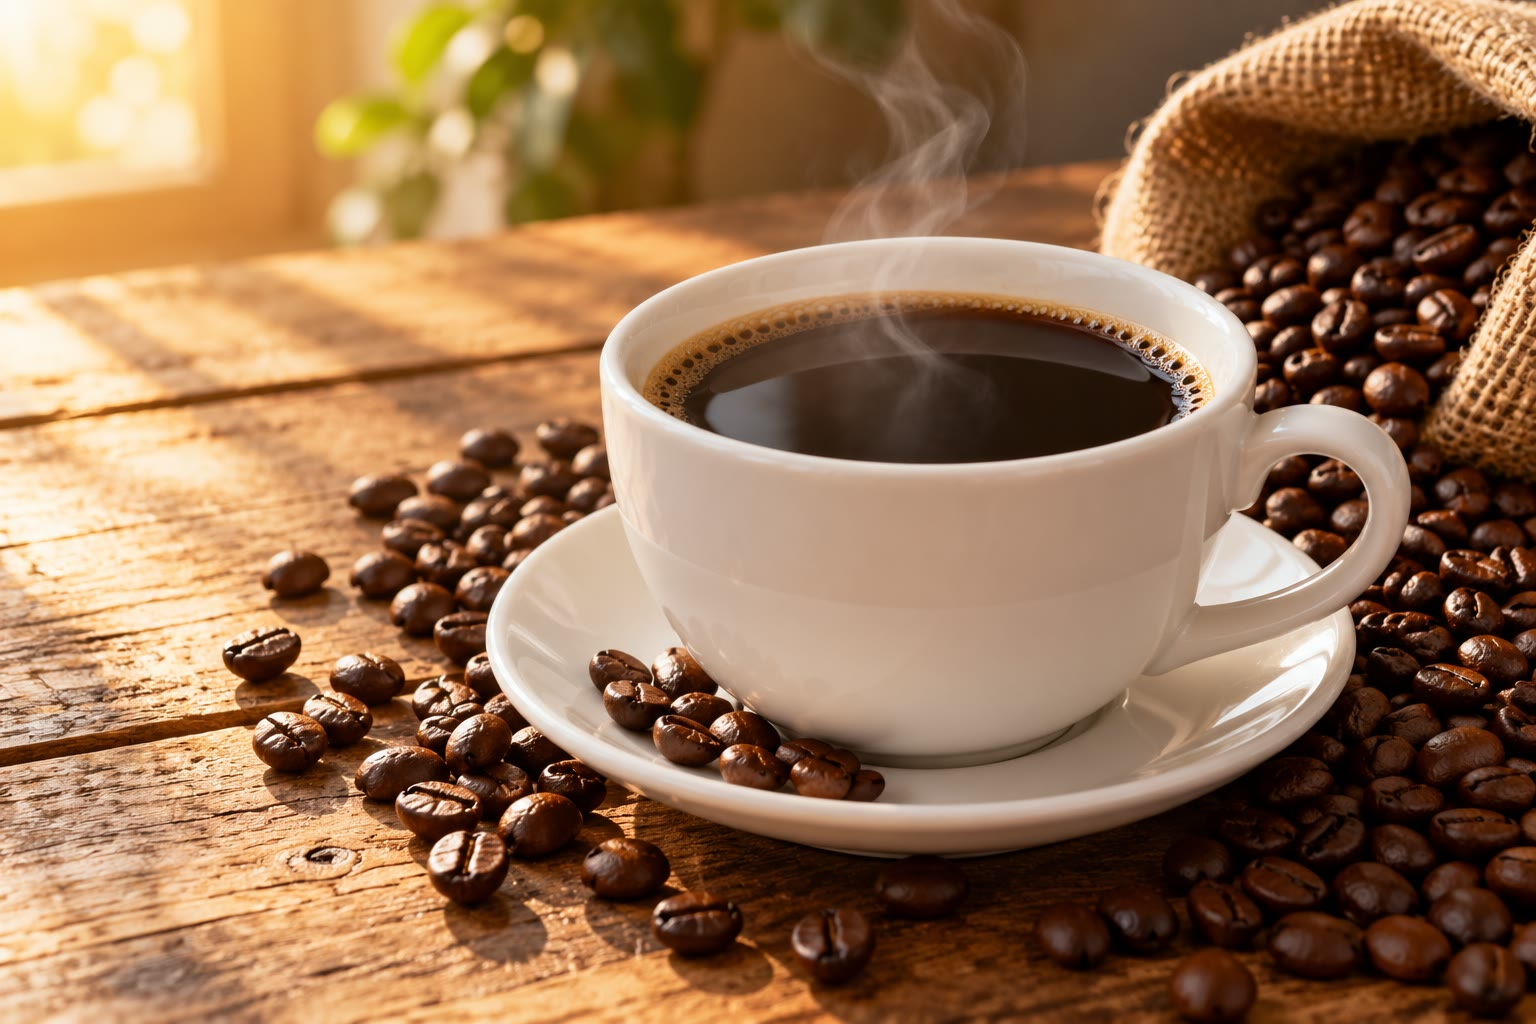
\includegraphics[width=0.5\linewidth]{images/book4/ai/b3-29-coffee.jpg}

{\small Una taza de café y granos tostados: la cafeína, una purina, y muchas de las
moléculas aromáticas formadas durante el tostado son \omterm{def:b3:heterocycles:heterocycle}{heterociclos}.}
\end{omfigure}

\section{Heterociclos aromáticos}

\begin{definition}[Heterociclos]\label{def:b3:heterocycles:heterocycle}
Un \emph{heterociclo}\index{heterociclo} es un compuesto cíclico con al menos un
átomo distinto del carbono en el anillo; un \emph{compuesto
heteroaromático}\index{compuesto heteroaromatico@compuesto heteroaromático} es uno aromático, como la piridina,
el pirrol, el furano o el tiofeno.
\end{definition}

\begin{proposition}[Seis electrones $\pi$]\label{prop:b3:heterocycles:sextet}
La piridina, el pirrol, el furano, el tiofeno y el imidazol tienen cada uno seis electrones $\pi$ en
un anillo plano, cíclico y conjugado, y son aromáticos según la regla de Hückel.
\end{proposition}

\begin{proof}
Piridina: cada uno de los cinco carbonos y el nitrógeno aporta un electrón p; el par
solitario del nitrógeno está en un orbital $sp^2$ en el plano del anillo, fuera del sistema $\pi$: $5 + 1 = 6$.
Pirrol: los cuatro carbonos aportan uno cada uno, y el nitrógeno, unido a un H en el plano,
pone su par solitario en su orbital p: $4 + 2 = 6$. Furano y tiofeno: como el pirrol, el
heteroátomo aporta uno de sus dos pares solitarios (el otro está en el plano). Imidazol:
el nitrógeno N--H aporta dos; el nitrógeno de tipo piridina, uno, y los tres carbonos,
tres: 6. Seis es $4n + 2$ con $n = 1$.
\end{proof}

\begin{omfigure}
\begin{tikzpicture}[font=\small, yscale=0.55]
  % pyridine: six p orbitals perpendicular to the ring (drawn first), N at 0 deg
  \foreach \a in {0,60,...,300} { \pic at (\a:1.1) {omp={0.62}{90}}; }
  \draw[thick] (0:1.1) -- (60:1.1) -- (120:1.1) -- (180:1.1) -- (240:1.1) -- (300:1.1) -- cycle;
  \node[fill=white, inner sep=0.5pt] at (0:1.1) {N};
  \pic at ($(0:1.1)+(0.2,0)$) {omlobe={0.8}{0}};
  \node[font=\scriptsize, align=center, anchor=north] at (0,-2.4) {piridina: 6 electrones p de 6 átomos;\\ par solitario en el plano (básico)};
  \begin{scope}[xshift=5.4cm]
    \foreach \a in {0,72,144,216,288} { \pic at (\a:1.0) {omp={0.62}{90}}; }
    \draw[thick] (0:1.0) -- (72:1.0) -- (144:1.0) -- (216:1.0) -- (288:1.0) -- cycle;
    \node[fill=white, inner sep=0.5pt] at (0:1.0) {N};
    \draw ($(0:1.0)+(0.18,0)$) -- (0:1.7) node[right, inner sep=0.5pt] {H};
    \node[font=\scriptsize, align=center, anchor=north] at (0,-2.4) {pirrol: el par solitario del N es uno de\\ los 6 electrones $\pi$ (no básico)};
  \end{scope}
\end{tikzpicture}

{\small Los sistemas $\pi$ de la piridina y del pirrol, vistos en perspectiva: un orbital p por
átomo del anillo, perpendicular al anillo. En la piridina, el par solitario del nitrógeno (el lóbulo en el plano, sobre el
nitrógeno) apunta hacia fuera en el plano del anillo y está libre para unir un protón; en el pirrol,
el nitrógeno, que lleva un hidrógeno en el plano, cede su par solitario al
sexteto aromático.}
\end{omfigure}

\begin{definition}[Heterociclos $\pi$-excedentes y $\pi$-deficientes]\label{def:b3:heterocycles:pi-character}
Un \emph{heterociclo $\pi$-excedente}\index{heterociclo $\pi$-excedente}, como el
pirrol, el furano o el tiofeno, tiene seis electrones $\pi$ sobre cinco átomos y una
\omterm{def:b3:computational-chemistry:dft}{densidad electrónica} $\pi$ en sus carbonos mayor que la del benceno; un \emph{heterociclo
$\pi$-deficiente}\index{heterociclo $\pi$-deficiente}, como la piridina, tiene un
átomo electronegativo en el anillo que retira densidad $\pi$ de los carbonos.
\end{definition}

\begin{proposition}[Basicidad]\label{prop:b3:heterocycles:basicity}
La piridina es una base moderada, y el pirrol, casi ninguna; el pirrol, cuando se
protona en un ácido fuerte, toma el protón en un carbono, no en el nitrógeno.
\end{proposition}

\begin{proof}[Argumento]
% ledger: pka:pyridinium, pka4:pyrrolium, pka4:piperidinium, pka4:imidazolium, pka4:DMAPH
El par solitario de la piridina está fuera del sistema $\pi$: protonarlo no cuesta
aromaticidad, y el piridinio tiene $\mathrm pK_a = 5.2$; es menos básica que la piperidina
(el nitrógeno del piridinio es $sp^2$, con más carácter s, y retiene su par con más
fuerza: piperidinio, 11.1). Protonar el nitrógeno del pirrol sacaría su par
solitario del sexteto y destruiría la aromaticidad; solo los ácidos muy fuertes
protonan el pirrol, y lo hacen en C2, donde el catión conserva cierta deslocalización
($\mathrm pK_a$ de alrededor de $-4$). El imidazol tiene los dos tipos de nitrógeno: se protona en el
de tipo piridina, y su catión, simétrico, está estabilizado por resonancia ($\mathrm pK_a$
7.0), la razón por la que la histidina actúa como ácido y como base en las \omterm{def:b3:complex-kinetics:enzyme}{enzimas}.
La 4-(dimetilamino)piridina es más básica aún ($\mathrm pK_a$ 9.6): el grupo amino empuja
su par solitario hacia el anillo y hasta el nitrógeno del anillo.
\end{proof}

% ledger: dip:pyridine, dip4:pyrrole, dip4:furan, dip4:thiophene
Los momentos dipolares cuentan la misma historia: la piridina (\qty{2.19}{D}) tiene su extremo negativo
en el nitrógeno, mientras que en el pirrol (\qty{1.84}{D}) la cesión del par solitario al anillo
sitúa el extremo negativo en el anillo y el positivo en el nitrógeno. En el furano
(\qty{0.66}{D}) y el tiofeno (\qty{0.55}{D}), los dos efectos, la atracción $\sigma$ y la donación $\pi$, casi
se compensan.

\begin{omfigure}
% ledger: h1:pyridine.a, h1:pyridine.g, h1:pyridine.b, h1:pyrrole.a, h1:pyrrole.b, h1:pyrrole.NH, h1:furan.a, h1:furan.b
\begin{tikzpicture}
\begin{axis}[width=0.86\linewidth, height=6.2cm, x dir=reverse, xmin=5.8, xmax=9.0, ymin=-0.1, ymax=3.6,
  axis x line=bottom, axis y line=none, xlabel={$\delta$ / ppm}, tick label style={font=\scriptsize}, label style={font=\small}]
\addplot[omDef, thick] table[x=ppm, y expr=\thisrow{y}+2.4] {figdata/out/bachelor-3-heterocycle-nmr-pyridine.dat};
\addplot[omThm, thick] table[x=ppm, y expr=\thisrow{y}+1.2] {figdata/out/bachelor-3-heterocycle-nmr-pyrrole.dat};
\addplot[omMeth, thick] table[x=ppm, y=y] {figdata/out/bachelor-3-heterocycle-nmr-furan.dat};
\node[font=\scriptsize, omDef, anchor=west] at (axis cs:7.1,3.0) {piridina: H2/6, H4, H3/5 (2\,:\,1\,:\,2)};
\node[font=\scriptsize, omThm, anchor=west] at (axis cs:7.7,1.8) {pirrol: NH, H2/5, H3/4};
\node[font=\scriptsize, omMeth, anchor=west] at (axis cs:7.2,0.6) {furano: H2/5, H3/4};
\end{axis}
\end{tikzpicture}

{\small RMN de protón de la piridina, el pirrol y el furano en deuterocloroformo,
sintetizada a partir de desplazamientos medidos como rayas simples (sin acoplamientos), con
áreas iguales al número de protones. La piridina, $\pi$-deficiente, tiene sus señales H2/6 y H4
muy a campo bajo respecto de la del benceno; el pirrol y el furano, $\pi$-excedentes, tienen la mayoría
de las suyas a campo alto respecto de ella; los protones contiguos al heteroátomo son siempre los más
desapantallados.}
\end{omfigure}

\section{La piridina}

La piridina resiste la sustitución electrófila: el electrófilo encuentra un anillo
más pobre en electrones que el benceno y, en el ácido que suele estar presente, un
ion piridinio cuya carga positiva lo repele. La nitración exige condiciones muy
drásticas y da el isómero 3 con un rendimiento bajo.

\begin{proposition}[Sustitución electrófila en C3]\label{prop:b3:heterocycles:pyridine-c3}
El ataque electrófilo sobre la piridina se produce en C3: el ataque en C2 o en C4 da un
intermedio de Wheland una de cuyas estructuras resonantes sitúa la carga
positiva en el nitrógeno, con solo seis electrones a su alrededor.
\end{proposition}

\begin{proof}
En el catión procedente del ataque en C2 (o en C4), la carga positiva se reparte entre C3, C5
y N1 (o C3, C5 y N1): una estructura resonante con un nitrógeno deficiente en electrones,
de seis electrones, muy desfavorable para un átomo electronegativo. El ataque
en C3 reparte la carga solo entre C2, C4 y C6. Los tres cationes son menos estables
que el del benceno, pero el ataque en C3 es el menos malo.
\end{proof}

\begin{definition}[N-óxido de piridina]\label{def:b3:heterocycles:n-oxide}
Un \emph{N-óxido de piridina}\index{N-oxido de piridina@N-óxido de piridina}, que se obtiene oxidando la piridina
con un peroxiácido, tiene un grupo $\mathrm{N^+{-}O^-}$ cuyo oxígeno devuelve electrones a C2
y C4; experimenta la sustitución electrófila en C4, y después se elimina el
oxígeno.
\end{definition}

\begin{definition}[Sustitución nucleófila aromática]\label{def:b3:heterocycles:snar}
La \emph{sustitución nucleófila aromática}\index{sustitucion nucleofila aromatica@sustitución nucleófila aromática}
($\mathrm S_\mathrm NAr$) sustituye un grupo saliente de un anillo aromático pobre en electrones
por un nucleófilo, mediante una adición seguida de una eliminación. El intermedio
aniónico de adición es un \emph{complejo de Meisenheimer}\index{complejo de Meisenheimer}.
\end{definition}

\begin{proposition}[$\mathrm S_\mathrm NAr$ en C2 y C4]\label{prop:b3:heterocycles:snar-positions}
Las halopiridinas experimentan fácilmente la $\mathrm S_\mathrm NAr$ en C2 y C4, y solo lentamente en C3,
porque la adición en C2 o C4 sitúa la carga negativa en el nitrógeno.
\end{proposition}

\begin{proof}
La adición en C2 hace $sp^3$ a C2 y deja cuatro electrones $\pi$ más el par entrante
repartidos sobre N1, C3 y C5 (o, para C4: C3, C5 y N1): una estructura resonante tiene la
carga negativa en el nitrógeno, electronegativo. La adición en C3 la reparte solo sobre
C2, C4 y C6, todos carbonos.
\end{proof}

\begin{omfigure}
\begin{tikzpicture}[font=\small, >=Stealth]
  \draw[thick] (-0.000,-0.620) -- (0.537,-0.310) -- (0.537,0.310) -- (0.000,0.620) -- (-0.537,0.310) -- (-0.537,-0.310) -- cycle;
  \draw[thick] (0.082,-0.424) -- (0.326,-0.283);
  \draw[thick] (0.326,0.283) -- (0.082,0.424);
  \draw[thick] (-0.408,0.141) -- (-0.408,-0.141);
  \node[fill=white, inner sep=0.4pt, font=\scriptsize] at (-0.000,-0.620) {N};
  \draw (0.537,-0.310) -- (0.927,-0.535) node[right, inner sep=0.5pt, font=\scriptsize] {Cl};
  \draw[thick] (3.400,-0.620) -- (3.937,-0.310) -- (3.937,0.310) -- (3.400,0.620) -- (2.863,0.310) -- (2.863,-0.310) -- cycle;
  \draw[thick] (3.726,0.283) -- (3.482,0.424);
  \draw[thick] (2.992,0.141) -- (2.992,-0.141);
  \node[fill=white, inner sep=0.4pt, font=\scriptsize] at (3.400,-0.620) {N};
  \node[font=\scriptsize, omThm] at (3.350,-0.920) {$\ominus$};
  \draw (3.937,-0.310) -- (4.386,-0.343) node[right, inner sep=0.5pt, font=\scriptsize] {Nu};
  \draw (3.937,-0.310) -- (4.190,-0.682) node[right, inner sep=0.5pt, font=\scriptsize] {Cl};
  \draw[thick] (6.800,-0.620) -- (7.337,-0.310) -- (7.337,0.310) -- (6.800,0.620) -- (6.263,0.310) -- (6.263,-0.310) -- cycle;
  \draw[thick] (6.882,-0.424) -- (7.126,-0.283);
  \draw[thick] (7.126,0.283) -- (6.882,0.424);
  \draw[thick] (6.392,0.141) -- (6.392,-0.141);
  \node[fill=white, inner sep=0.4pt, font=\scriptsize] at (6.800,-0.620) {N};
  \draw (7.337,-0.310) -- (7.727,-0.535) node[right, inner sep=0.5pt, font=\scriptsize] {Nu};
  \draw[->, thick] (1.25,0) -- (2.35,0) node[midway, above, font=\scriptsize] {$+\,\mathrm{Nu^-}$};
  \draw[->, thick] (4.65,0) -- (5.75,0) node[midway, above, font=\scriptsize] {$-\,\ce{Cl-}$};
  \node[font=\scriptsize] at (3.4,-1.2) {complejo de Meisenheimer};
\end{tikzpicture}

{\small Sustitución nucleófila de la 2-cloropiridina: el nucleófilo se adiciona a
C2, lo que da un intermedio aniónico cuya carga negativa reside en gran parte en el
nitrógeno del anillo (se muestra una estructura resonante); después sale el cloruro y se
restablece el anillo aromático.}
\end{omfigure}

\begin{proposition}[Adición--eliminación]\label{prop:b3:heterocycles:snar-mechanism}
Para una reacción $\mathrm S_\mathrm NAr$ cuya etapa de adición es determinante de la velocidad, $v = k[\mathrm{ArX}][\mathrm{Nu^-}]$,
y el fluoruro es el mejor grupo saliente entre los haluros.
\end{proposition}

\begin{proof}[Argumento]
La velocidad es la de la adición bimolecular. El enlace carbono--halógeno no se
rompe en esa etapa; lo que importa es cuánto rebaja el halógeno la energía del
estado de transición aniónico al atraer electrones, y el flúor, el más
electronegativo, es el que más la rebaja: el orden F $>$ Cl $\approx$ Br $>$ I, opuesto al de la $\mathrm S_\mathrm N2$.
\end{proof}

\begin{definition}[Reacción de Chichibabin]\label{def:b3:heterocycles:chichibabin}
La \emph{reacción de Chichibabin}\index{reaccion de Chichibabin@reacción de Chichibabin} es la aminación de
la piridina en C2 con amiduro de sodio: el ion amiduro se adiciona a C2, y se pierde
un ion hidruro, en forma de dihidrógeno tras reaccionar con el producto.
\end{definition}

La piridina y la DMAP sirven también como bases y como catalizadores nucleófilos: en
las acilaciones con anhídridos de ácido, la DMAP ataca primero el anhídrido y da un
ion acilpiridinio que transfiere su grupo acilo al alcohol mucho más deprisa que
el propio anhídrido. Las piridinas, las bipiridinas y las fenantrolinas figuran entre los
ligandos más comunes de la química de coordinación.

\section{Anillos de cinco miembros}

\begin{proposition}[Sustitución electrófila del pirrol en C2]\label{prop:b3:heterocycles:pyrrole-c2}
El pirrol, el furano y el tiofeno experimentan la sustitución electrófila principalmente en C2,
porque el catión procedente del ataque en C2 tiene tres estructuras resonantes, y el
procedente del ataque en C3, solo dos.
\end{proposition}

\begin{proof}
Tras el ataque en C2, la carga positiva puede situarse en C3, en C5 o en el nitrógeno,
donde se comparte a través del par solitario y todos los átomos conservan el octeto (tercera
estructura). Tras el ataque en C3, solo puede situarse en C2 o en el nitrógeno: la carga
está menos deslocalizada (véase la figura).
\end{proof}

\begin{omfigure}
\begin{tikzpicture}[font=\small]
  \draw[thick] (0.000,0.620) -- (0.590,0.192) -- (0.364,-0.502) -- (-0.364,-0.502) -- (-0.590,0.192) -- cycle;
  \draw[thick] (-0.303,-0.269) -- (-0.403,0.039);
  \node[fill=white, inner sep=0.4pt, font=\scriptsize] at (0.000,0.620) {N};
  \draw (0.000,0.750) -- (0.000,1.020) node[above, inner sep=0.5pt, font=\scriptsize] {H};
  \draw (0.590,0.192) -- (0.893,0.482) node[right, inner sep=0.5pt, font=\scriptsize] {H};
  \draw (0.590,0.192) -- (1.006,0.135) node[right, inner sep=0.5pt, font=\scriptsize] {E};
  \node[font=\scriptsize, omThm] at (0.164,-0.226) {$\oplus$};
  \draw[thick] (2.600,0.620) -- (3.190,0.192) -- (2.964,-0.502) -- (2.236,-0.502) -- (2.010,0.192) -- cycle;
  \draw[thick] (2.762,-0.371) -- (2.438,-0.371);
  \node[fill=white, inner sep=0.4pt, font=\scriptsize] at (2.600,0.620) {N};
  \draw (2.600,0.750) -- (2.600,1.020) node[above, inner sep=0.5pt, font=\scriptsize] {H};
  \draw (3.190,0.192) -- (3.493,0.482) node[right, inner sep=0.5pt, font=\scriptsize] {H};
  \draw (3.190,0.192) -- (3.606,0.135) node[right, inner sep=0.5pt, font=\scriptsize] {E};
  \node[font=\scriptsize, omThm] at (2.335,0.086) {$\oplus$};
  \draw[thick] (5.200,0.620) -- (5.790,0.192) -- (5.564,-0.502) -- (4.836,-0.502) -- (4.610,0.192) -- cycle;
  \draw[thick] (5.362,-0.371) -- (5.038,-0.371);
  \draw[thick] (5.113,0.395) -- (4.851,0.205);
  \node[fill=white, inner sep=0.4pt, font=\scriptsize] at (5.200,0.620) {N};
  \draw (5.200,0.750) -- (5.200,1.020) node[above, inner sep=0.5pt, font=\scriptsize] {H};
  \draw (5.790,0.192) -- (6.093,0.482) node[right, inner sep=0.5pt, font=\scriptsize] {H};
  \draw (5.790,0.192) -- (6.206,0.135) node[right, inner sep=0.5pt, font=\scriptsize] {E};
  \node[font=\scriptsize, omThm] at (5.480,0.700) {$\oplus$};
  \draw[thick] (8.400,0.620) -- (8.990,0.192) -- (8.764,-0.502) -- (8.036,-0.502) -- (7.810,0.192) -- cycle;
  \draw[thick] (8.097,-0.269) -- (7.997,0.039);
  \node[fill=white, inner sep=0.4pt, font=\scriptsize] at (8.400,0.620) {N};
  \draw (8.400,0.750) -- (8.400,1.020) node[above, inner sep=0.5pt, font=\scriptsize] {H};
  \draw (8.764,-0.502) -- (9.135,-0.700) node[right, inner sep=0.5pt, font=\scriptsize] {H};
  \draw (8.764,-0.502) -- (8.839,-0.915) node[right, inner sep=0.5pt, font=\scriptsize] {E};
  \node[font=\scriptsize, omThm] at (8.665,0.086) {$\oplus$};
  \draw[thick] (11.000,0.620) -- (11.590,0.192) -- (11.364,-0.502) -- (10.636,-0.502) -- (10.410,0.192) -- cycle;
  \draw[thick] (10.697,-0.269) -- (10.597,0.039);
  \draw[thick] (11.087,0.395) -- (11.349,0.205);
  \node[fill=white, inner sep=0.4pt, font=\scriptsize] at (11.000,0.620) {N};
  \draw (11.000,0.750) -- (11.000,1.020) node[above, inner sep=0.5pt, font=\scriptsize] {H};
  \draw (11.364,-0.502) -- (11.735,-0.700) node[right, inner sep=0.5pt, font=\scriptsize] {H};
  \draw (11.364,-0.502) -- (11.439,-0.915) node[right, inner sep=0.5pt, font=\scriptsize] {E};
  \node[font=\scriptsize, omThm] at (11.280,0.700) {$\oplus$};
  \node[font=\scriptsize] at (2.6,-1.35) {ataque en C2: tres estructuras};
  \node[font=\scriptsize] at (9.7,-1.35) {ataque en C3: dos estructuras};
  \draw[black!40] (6.8,-1.2) -- (6.8,1.2);
\end{tikzpicture}

{\small Intermedios de Wheland del pirrol (E: el electrófilo; $\oplus$: carga positiva).
El ataque en C2 da un catión con la carga en C3, en C5 o en el nitrógeno con todos los
octetos completos; el ataque en C3, solo en C2 o en el nitrógeno.}
\end{omfigure}

El pirrol es aproximadamente tan reactivo como el fenol o la anilina: se broma, se nitra
y se acila en condiciones suaves, polimeriza en ácido fuerte y se
formila en C2 con el reactivo de Vilsmeier, obtenido a partir de dimetilformamida y oxicloruro de
fósforo. Las reactividades disminuyen en el orden pirrol $>$ furano $>$ tiofeno $>$ benceno,
según la disposición del heteroátomo a compartir su par solitario. El furano,
el menos aromático, reacciona también como dieno en reacciones de Diels--Alder. Las bases
fuertes, como el butillitio, desprotonan el furano y el tiofeno en C2, junto al
heteroátomo, y dan reactivos organolíticos.

\begin{method}[Predecir el sitio de ataque sobre un heterociclo]\label{met:b3:heterocycles:site}
\begin{enumerate}
  \item Clasificar el anillo: $\pi$-excedente (heteroátomo de tipo pirrol) o $\pi$-deficiente
        (nitrógeno de tipo piridina).
  \item Electrófilos: sobre un anillo $\pi$-excedente, en C2 (en C3 para el indol, cuyo ataque en C2
        alteraría el anillo bencénico); sobre la piridina, en C3, o en C4 a través del
        N-óxido.
  \item Nucleófilos: sobre un anillo $\pi$-deficiente, en C2 o C4, sobre todo si hay allí un grupo
        saliente.
  \item Bases fuertes: en el C--H contiguo al heteroátomo.
\end{enumerate}
\end{method}

\section{Heterociclos fusionados y biológicos}

El indol, un benceno fusionado con un pirrol, reacciona con los electrófilos en C3: allí, el
intermedio conserva intacto el anillo bencénico, con la carga en el nitrógeno.
La quinolina, un benceno fusionado con una piridina, es sustituida por los electrófilos en
su anillo bencénico y por los nucleófilos en C2 y C4. Las bases nitrogenadas son
pirimidinas (citosina, timina, uracilo) y purinas (adenina, guanina), una
pirimidina fusionada con un imidazol. Sus formas oxo y amino (tautómeros lactama y
amina) predominan sobre las formas hidroxi e imino, lo que fija el patrón de
dadores y aceptores de enlaces de hidrógeno de cada base y, por tanto, el apareamiento de bases.

\begin{omfigure}
\begin{tikzpicture}[font=\small]
  \node[draw, rounded corners, minimum width=1.8cm, minimum height=2.8cm, fill=omDef!8] at (0,0) {};
  \node[font=\small\bfseries] at (0,1.75) {guanina};
  \node[anchor=east] (g1) at (0.85,0.85) {C6=O};
  \node[anchor=east] (g2) at (0.85,0) {N1--H};
  \node[anchor=east] (g3) at (0.85,-0.85) {C2--N--H};
  \node[draw, rounded corners, minimum width=1.8cm, minimum height=2.8cm, fill=omThm!8] at (3.2,0) {};
  \node[font=\small\bfseries] at (3.2,1.75) {citosina};
  \node[anchor=west] (c1) at (2.35,0.85) {H--N--C4};
  \node[anchor=west] (c2) at (2.35,0) {N3};
  \node[anchor=west] (c3) at (2.35,-0.85) {O=C2};
  \draw[omMeth, very thick, dotted] (g1.east) -- (c1.west);
  \draw[omMeth, very thick, dotted] (g2.east) -- (c2.west);
  \draw[omMeth, very thick, dotted] (g3.east) -- (c3.west);
\end{tikzpicture}

{\small Un par de bases guanina--citosina, en esquema: tres enlaces de hidrógeno (en verde)
entre el oxígeno carbonílico de la guanina y un N--H amino de la citosina, el N1--H de
la guanina y el N3 del anillo de la citosina, y un N--H amino de la guanina y el
oxígeno carbonílico de la citosina. La adenina y la timina forman dos.}
\end{omfigure}

\section{Construir anillos}

\begin{definition}[Síntesis de Paal--Knorr]\label{def:b3:heterocycles:paal-knorr}
La \emph{síntesis de Paal--Knorr}\index{sintesis de Paal--Knorr@síntesis de Paal--Knorr} prepara un furano
(con ácido), un pirrol (con una amina primaria o con amoníaco) o un tiofeno (con un
reactivo de azufre) a partir de un compuesto 1,4-dicarbonílico.
\end{definition}

\begin{definition}[Síntesis de piridinas de Hantzsch]\label{def:b3:heterocycles:hantzsch}
La \emph{síntesis de piridinas de Hantzsch}\index{sintesis de piridinas de Hantzsch@síntesis de piridinas de Hantzsch}
condensa un aldehído, dos equivalentes de un $\beta$-cetoéster y amoníaco en una
1,4-dihidropiridina, que puede oxidarse a la piridina.
\end{definition}

\begin{definition}[Síntesis de indoles de Fischer]\label{def:b3:heterocycles:fischer-indole}
La \emph{síntesis de indoles de Fischer}\index{sintesis de indoles de Fischer@síntesis de indoles de Fischer} calienta la
fenilhidrazona de un aldehído o de una cetona con un catalizador ácido: la hidrazona
tautomeriza a una enhidrazina, que experimenta una \omterm{def:b3:pericyclic:families}{transposición sigmatrópica}
[3,3]; la ciclación y la pérdida de amoníaco dan el indol.
\end{definition}

\begin{omfigure}
\setchemfig{atom sep=1.8em}
\schemestart
\chemfig{*6(-=-=(-NH-[:30]N=[:-30](-[:-90]CH_3)-[:30]CH_3)-=)}
\arrow{->[$\ce{H+}$][tautómero]}[,1.4]
\chemfig{*6(-=-=(-NH-[:30]NH-[:-30](=[:-90]CH_2)-[:30]CH_3)-=)}
\schemestop
\par\bigskip
\schemestart
\arrow{->[{[3,3]}, después][ciclación, $-\ce{NH3}$]}[,2.2]
\chemfig{*6(-=*5(-=(-CH_3)-N(-H)-)-=-=)}
\schemestop

{\small La \omterm{def:b3:heterocycles:fischer-indole}{síntesis de indoles de Fischer} a partir de la fenilhidrazona de la acetona. El ácido convierte la
hidrazona en su tautómero enhidrazina; la transposición [3,3] rompe el enlace
N--N y forma un enlace C--C entre el carbono del anillo en \textit{orto} respecto del nitrógeno y el
$\ce{CH2}$ terminal; la nueva amina ataca la imina, y la pérdida de amoníaco da el
2-metilindol.}
\end{omfigure}

\begin{method}[Desconectar un heterociclo]\label{met:b3:heterocycles:disconnect}
\begin{enumerate}
  \item Un pirrol, un furano o un tiofeno 2,5-disustituidos: desconectar los dos enlaces con
        el heteroátomo y volver a una 1,4-dicetona (Paal--Knorr).
  \item Una 1,4-dihidropiridina simétrica con ésteres en C3 y C5: volver a un
        aldehído, dos $\beta$-cetoésteres y amoníaco (Hantzsch).
  \item Un indol 2,3-disustituido: volver a la fenilhidrazina y a la cetona
        $\mathrm{R^2CH_2COR^3}$ (Fischer).
  \item Comprobar la disponibilidad de las piezas y, después, la regioquímica cuando la cetona
        es asimétrica.
\end{enumerate}
\end{method}

\begin{definition}[Bioisóstero]\label{def:b3:heterocycles:bioisostere}
Un \emph{bioisóstero}\index{bioisostero@bioisóstero} es un grupo que sustituye a otro en una
molécula de fármaco conservando su actividad biológica, porque tiene un
tamaño, una forma y un patrón de enlaces de hidrógeno y de carga parecidos, como un tetrazol en
lugar de un ácido carboxílico, o una piridina en lugar de un anillo bencénico.
\end{definition}

\begin{inthelab}[Un pirrol de Paal--Knorr]
La hexano-2,5-diona, la anilina y una cantidad catalítica de ácido 4-toluenosulfónico se
calientan a reflujo en tolueno en un matraz provisto de una trampa de Dean--Stark: el
agua formada se arrastra como azeótropo y se acumula en el brazo lateral, lo que
lleva la condensación hasta el final. Cuando ya no se separa más agua, la
disolución se lava con hidrogenocarbonato de sodio acuoso, se seca y se evapora,
y el 2,5-dimetil-1-fenilpirrol se recristaliza.
\end{inthelab}

\begin{safety}{\ghs[0.62cm]{GHS02}\ghs[0.62cm]{GHS06}\ghs[0.62cm]{GHS07}\ghs[0.62cm]{GHS08}\ghs[0.62cm]{GHS09}}
% ledger: ghs4:pyridine, ghs4:phenylhydrazine
Piridina: muy inflamable, nociva por todas las vías, de olor intenso; se usa en una
vitrina. Fenilhidrazina: tóxica por todas las vías, puede provocar cáncer y defectos
genéticos, perjudica a la sangre por exposición prolongada, sensibilizante, muy tóxica para los
organismos acuáticos; se pesa en una vitrina con guantes, y sus residuos se recogen
por separado.
\end{safety}

\begin{history}[Dos síntesis clásicas de anillos]
Emil Fischer describió su síntesis de indoles en 1883, en los mismos años que sus
trabajos sobre los azúcares y las purinas; Arthur Hantzsch publicó su síntesis de piridinas
en 1881. Ambas siguen en uso: la síntesis de Fischer para los
triptanes contra la migraña, y la de Hantzsch para las dihidropiridinas
bloqueadoras de los canales de calcio que tratan la hipertensión arterial.
\end{history}

\section{Ejercicios}

\begin{exercise}[$\star$]\label{exo:b3:heterocycles:1}
Cuéntense los electrones $\pi$ del oxazol, el tiazol, la pirimidina y la purina, y dígase qué
pares solitarios pertenecen al sistema $\pi$.
\end{exercise}

\begin{exercise}[$\star$]\label{exo:b3:heterocycles:2}
Ordénense la piridina, el pirrol, el imidazol, la piperidina y la DMAP por basicidad, con sus
valores de $\mathrm pK_a$.
\end{exercise}

\begin{exercise}[$\star$]\label{exo:b3:heterocycles:3}
Dese el producto principal de la monobromación del pirrol, del furano y del indol.
\end{exercise}

\begin{exercise}[$\star$]\label{exo:b3:heterocycles:4}
Dense los productos de la reacción de Paal--Knorr de la hexano-2,5-diona con ácido solo,
con metilamina y con pentasulfuro de fósforo.
\end{exercise}

\begin{exercise}[$\star\star$]\label{exo:b3:heterocycles:5}
La 2-cloropiridina reacciona con metóxido de sodio en metanol a \qty{65}{\celsius}; la 3-cloropiridina
apenas lo hace. Explíquese y dese el producto.
\end{exercise}

\begin{exercise}[$\star\star$]\label{exo:b3:heterocycles:6}
Dese el producto de la \omterm{def:b3:heterocycles:chichibabin}{reacción de Chichibabin} de la piridina y dibújese el intermedio
de adición.
\end{exercise}

\begin{exercise}[$\star\star$]\label{exo:b3:heterocycles:7}
El \omterm{def:b3:heterocycles:n-oxide}{N-óxido de piridina} se nitra en C4. Explíquese con estructuras resonantes, y dígase cómo
se obtiene la 4-nitropiridina.
\end{exercise}

\begin{exercise}[$\star\star$]\label{exo:b3:heterocycles:8}
La 2-hidroxipiridina existe en agua principalmente como 2-piridona. Dibújense los dos tautómeros y
explíquese por qué la piridona sigue siendo aromática.
\end{exercise}

\begin{exercise}[$\star\star$]\label{exo:b3:heterocycles:9}
Dense los componentes de una síntesis de Hantzsch de la 1,4-dihidropiridina con
ésteres metílicos en C3 y C5, grupos metilo en C2 y C6 y un grupo 2-nitrofenilo
en C4.
\end{exercise}

\begin{exercise}[$\star\star\star$]\label{exo:b3:heterocycles:10}
La butanona da dos indoles distintos en la síntesis de Fischer con
fenilhidrazina. Dense ambos, y dígase cómo cambia su proporción la fuerza del ácido.
\end{exercise}

\begin{exercise}[$\star\star\star$]\label{exo:b3:heterocycles:11}
Explíquese por qué el 4-fluoronitrobenceno y la 2-fluoropiridina reaccionan más deprisa con los
nucleófilos que los cloruros correspondientes, a diferencia de los sustratos de $\mathrm S_\mathrm N2$.
\end{exercise}

\begin{exercise}[$\star\star\star$]\label{exo:b3:heterocycles:12}
Con los espectros sintéticos del capítulo, explíquese cómo se distinguirían la piridina,
el pirrol y el furano por su RMN de protón, y predígase el espectro del
tiofeno (desplazamientos de \qty{7.33}{ppm} y \qty{7.12}{ppm}).
\end{exercise}

\section{Problema: construir un indol}

\begin{problem}[{Problema de fin de semana --- construir un indol: la fenilhidrazona de la
acetona, la enhidrazina y su transposición [3,3], la pérdida de amoníaco
y la elección entre dos indoles con la butanona}]
\label{pb:b3:heterocycles:1}
% ledger: aw:C, aw:H, aw:N, aw:O
Datos del problema: 10.0 g de fenilhidrazina reaccionan con un exceso de acetona, y
la hidrazona se calienta con cloruro de cinc.

\medskip\noindent\textbf{Parte I --- La hidrazona.}
\begin{enumerate}
  \item Escríbase la formación de la fenilhidrazona de la acetona.
  \item ¿Por qué es una condensación de tipo imina, y por qué es útil una traza de ácido?
  \item ¿Qué nitrógeno de la fenilhidrazina ataca el grupo carbonilo, y por qué?
  \item Calcúlense la masa molar de la fenilhidrazina y la cantidad usada.
  \item Calcúlese la masa teórica de hidrazona.
\end{enumerate}

\medskip\noindent\textbf{Parte II --- La enhidrazina y la etapa [3,3].}
\begin{enumerate}[resume]
  \item Dibújese el tautómero enhidrazina.
  \item ¿Qué seis átomos forman el estado de transición cíclico de la transposición [3,3]?
  \item ¿Qué enlace se rompe y cuál se forma?
  \item ¿Cuántos electrones intervienen, y está permitida la etapa por vía térmica?
  \item ¿Qué hace el cloruro de cinc?
  \item ¿Por qué tiene que restablecerse después la aromaticidad del anillo bencénico?
\end{enumerate}

\medskip\noindent\textbf{Parte III --- El cierre del anillo.}
\begin{enumerate}[resume]
  \item ¿Qué amina ataca a qué carbono para cerrar el anillo de cinco miembros?
  \item ¿Qué molécula pequeña se va, y qué impulsa la última etapa?
  \item Escríbase la ecuación global, de la hidrazona al 2-metilindol.
  \item Calcúlese la masa molar del 2-metilindol.
  \item Calcúlese la masa teórica de 2-metilindol.
  \item ¿Dónde sustituiría un electrófilo al 2-metilindol, y por qué?
\end{enumerate}

\medskip\noindent\textbf{Parte IV --- La butanona.}
\begin{enumerate}[resume]
  \item Dibújense las dos enhidrazinas de la fenilhidrazona de la butanona.
  \item Dense los dos indoles a los que conducen.
  \item ¿Qué enhidrazina está más sustituida, y cuál se forma en ácido fuerte?
  \item ¿Qué indol predomina con un ácido débil, y por qué?
  \item ¿Por qué la fenilhidrazona del acetaldehído no puede dar bien el propio indol?
  \item ¿Qué significa el problema de regioquímica para la síntesis de un fármaco?
  \item Enúnciese el resultado: la masa teórica de 2-metilindol obtenida a partir de 10.0 g de
        fenilhidrazina.
\end{enumerate}
\end{problem}
